\chapter{Stochastic Mesoscopic Equations}
\label{ch:stochastic-mesoscopic-equations}

\textit{A stochastic mesoscopic equation says that cluster activity follows a deterministic population drift plus finite-size fluctuations whose amplitude and covariance are part of the model. This chapter develops the language needed to distinguish noise-driven switching among stable states from deterministic irregular dynamics at the population level.}

% ============================================================
\section{Langevin descriptions of population activity}
\label{sec:langevin-population-activity}
% ============================================================

A Langevin equation describes the time evolution of a state variable with both deterministic drift and stochastic fluctuations. For $P$ mesoscopic populations, write the state as
%
\begin{equation}
  \vec R(t)
  =
  (R_1(t),\ldots,R_P(t))^\top,
  \label{eq:mesoscopic-state-vector}
\end{equation}
%
where $R_\alpha$ may be the filtered activity of cluster $\alpha$, an excitatory subcluster, or an inhibitory subcluster.

The generic stochastic mesoscopic equation is
%
\begin{keyequation}[Mesoscopic Langevin Equation]
\begin{equation}
  \dd \vec R
  =
  \vec f(\vec R;\theta)\,\dd t
  +
  \frac{1}{\sqrt{N}}\,
  \mat G(\vec R;\theta)\,\dd \vec W_t .
  \label{eq:mesoscopic-langevin}
\end{equation}
\tcblower
$\vec f$: deterministic population drift; \quad
$\theta$: model parameters; \quad
$N$: population-size scale; \quad
$\mat G$: noise-amplitude matrix; \quad
$\vec W_t$: independent Wiener processes before mixing by $\mat G$.
\end{keyequation}

\noindent The drift $\vec f$ contains leak, recurrent excitation, inhibition, external input, adaptation, and any deterministic synaptic variables retained in the reduction. The stochastic term represents finite-size deviations between expected and realized population activity.

For a rate-based drift, one common form is
%
\begin{equation}
  f_\alpha(\vec R)
  =
  \frac{1}{\tau_\alpha}
  \left[
    -R_\alpha
    +
    \Phi_\alpha\!\left(
      I_\alpha
      +
      \sum_{\beta=1}^P W_{\alpha\beta}R_\beta
    \right)
  \right].
  \label{eq:stochastic-rate-drift}
\end{equation}
%
This deterministic part decides which fixed points and basins exist. The noise part decides how a finite network wanders around those basins and occasionally escapes them.

The associated diffusion matrix is
%
\begin{equation}
  \mat D(\vec R)
  =
  \frac{1}{2N}\,
  \mat G(\vec R)\mat G(\vec R)^\top .
  \label{eq:ch09-diffusion-matrix}
\end{equation}
%
It sets the covariance of small stochastic increments. If $\mat D$ has a large eigenvalue along a cluster-switching direction, transitions are much easier than the scalar noise amplitude alone would suggest.

% ============================================================
\section{Intrinsic noise from finite population size}
\label{sec:intrinsic-noise-finite-population-size}
% ============================================================

Intrinsic noise is generated by the finite number of neurons in a population. Even if the input and parameters are identical across trials, the realized spike count fluctuates because spikes are discrete events.

In a small bin $\Delta t$, suppose population $\alpha$ has conditional rate $r_\alpha(t)$. Under the simplest conditionally independent Poisson approximation,
%
\begin{equation}
  K_\alpha(t,\Delta t)
  \sim
  \operatorname{Poisson}\!\left(N_\alpha r_\alpha(t)\Delta t\right).
  \label{eq:population-count-poisson}
\end{equation}
%
The binned activity estimate is
%
\begin{equation}
  \widehat A_\alpha(t;\Delta t)
  =
  \frac{K_\alpha(t,\Delta t)}{N_\alpha\Delta t}.
  \label{eq:stochastic-binned-activity}
\end{equation}
%
It has mean and variance
%
\begin{equation}
  \E[\widehat A_\alpha]
  =
  r_\alpha,
  \qquad
  \Var[\widehat A_\alpha]
  =
  \frac{r_\alpha}{N_\alpha\Delta t}.
  \label{eq:intrinsic-noise-variance}
\end{equation}
%
This equation is the local origin of the $N_\alpha^{-1/2}$ scaling. The finite population activity is an unbiased estimate of the rate, but its standard deviation shrinks only as the square root of population size.

For multiple populations, intrinsic noise has a covariance matrix. In a bin,
%
\begin{equation}
  \operatorname{Cov}(\widehat A_\alpha,\widehat A_\beta)
  =
  \frac{1}{N_\alpha N_\beta\Delta t^2}
  \operatorname{Cov}(K_\alpha,K_\beta).
  \label{eq:activity-covariance-counts}
\end{equation}
%
If populations spike independently given their rates, this covariance is zero for $\alpha\ne\beta$. In recurrent networks it is often not zero, because populations share input and drive each other.

The intrinsic-noise hypothesis makes a strong prediction: after matching deterministic parameters, increasing the number of neurons per cluster should reduce fluctuations in $R_\alpha$ and should reduce the rate of noise-driven transitions.

% ============================================================
\section{Multiplicative noise in spiking populations}
\label{sec:multiplicative-noise-spiking-populations}
% ============================================================

Noise is called multiplicative when its amplitude depends on the current state. Population spiking noise is naturally multiplicative because the variance of spike count depends on rate.

A one-population diffusion approximation to binned Poisson activity is
%
\begin{equation}
  \dd R
  =
  f(R)\,\dd t
  +
  \frac{1}{\sqrt{N}}\,
  \sigma(R)\,\dd W_t,
  \qquad
  \sigma^2(R)\propto \Phi(H(R)).
  \label{eq:multiplicative-noise-one-pop}
\end{equation}
%
The factor $\sigma(R)$ is larger when the population is expected to emit more spikes. In an up-state, absolute spike-count fluctuations may be larger than in a down-state, even if relative fluctuations are smaller.

For a vector of populations, the covariance of stochastic increments over a small time step is
%
\begin{equation}
  \E[\dd R_\alpha\,\dd R_\beta\mid \vec R]
  =
  \frac{1}{N}
  \left[
    \mat G(\vec R)\mat G(\vec R)^\top
  \right]_{\alpha\beta}
  \dd t.
  \label{eq:multiplicative-noise-covariance}
\end{equation}
%
The diagonal entries give variance within each population. The off-diagonal entries give shared fluctuations.

Multiplicative noise changes escape behavior. A barrier that is high in deterministic phase space may still be crossed often if the noise covariance is large along the escape direction. Conversely, a nearby saddle may be rarely crossed if the noise is weak in the direction leading to it.

When analyzing a clustered model, it is therefore not enough to draw the deterministic basins. One should also ask how $\mat G(\vec R)$ projects onto the directions that connect cluster states.

% ============================================================
\section{Quenched disorder vs dynamic noise}
\label{sec:quenched-disorder-vs-dynamic-noise}
% ============================================================

Finite networks contain two different kinds of randomness.

\emph{Dynamic noise} changes across time and across repeated trials. Spike-count fluctuations, stochastic synaptic release, and random escape events are dynamic. In equations, dynamic noise appears as $\dd \vec W_t$ or as random point-process increments.

\emph{Quenched disorder} is fixed within a network realization. Random connectivity, fixed synaptic weights, threshold heterogeneity, and cluster-size imbalances are quenched. In equations, quenched disorder appears as fixed random parameters:
%
\begin{equation}
  W_{\alpha\beta}^{(m)}
  =
  \bar W_{\alpha\beta}
  +
  \Delta W_{\alpha\beta}^{(m)},
  \label{eq:quenched-disorder-network-m}
\end{equation}
%
where $m$ indexes the network realization. The term $\Delta W_{\alpha\beta}^{(m)}$ is random across networks but fixed during one simulation.

The distinction matters for metastability. Dynamic noise can make the same network leave a state at different times on repeated trials. Quenched disorder can make one state systematically more stable than another in every trial of the same network.

A useful decomposition of a measured cluster activity is
%
\begin{equation}
  R_\alpha^{(m,\ell)}(t)
  =
  \bar R_\alpha(t)
  +
  Q_\alpha^{(m)}(t)
  +
  \epsilon_\alpha^{(m,\ell)}(t),
  \label{eq:quenched-dynamic-decomposition}
\end{equation}
%
where $m$ indexes network realization and $\ell$ indexes trial. The term $Q_\alpha^{(m)}$ is realization-specific bias. The term $\epsilon_\alpha^{(m,\ell)}$ is trial-specific dynamic fluctuation.

To estimate these components, compare many trials of the same network with many independently drawn networks. If variability is mostly quenched, trial averages differ strongly across network realizations. If variability is mostly dynamic, repeated trials of the same network remain highly variable.

% ============================================================
\section{Annealed approximations}
\label{sec:annealed-approximations}
% ============================================================

An annealed approximation replaces fixed disorder by randomness that is averaged or resampled. For example, instead of simulating one fixed adjacency matrix, one may replace it by its connection probability and average weight:
%
\begin{equation}
  J_{ij}
  \quad\longrightarrow\quad
  \E[J_{ij}]
  =
  p_{\alpha\beta}j_{\alpha\beta}
  \qquad
  (i\in\alpha,\;j\in\beta).
  \label{eq:annealed-connectivity}
\end{equation}
%
This produces a cleaner mean-field equation, but it removes realization-specific biases.

A more refined annealed approximation keeps the variance of random connectivity as an additional dynamic noise source:
%
\begin{equation}
  H_\alpha(t)
  =
  I_\alpha(t)
  +
  \sum_\beta \bar W_{\alpha\beta}R_\beta(t)
  +
  \eta_\alpha^{\mathrm{ann}}(t),
  \label{eq:annealed-input-noise}
\end{equation}
%
where $\eta_\alpha^{\mathrm{ann}}$ is chosen to match the input variance caused by random wiring. This can be useful for predicting average statistics over network realizations.

The risk is conceptual. Quenched disorder and dynamic noise do not have the same effect on attractor landscapes. A fixed connectivity bias changes the drift field and can deepen one basin. Annealed noise shakes the system but does not create a persistent preference unless its statistics depend on state.

For this rotation, annealed approximations are useful as baselines. They answer: what would happen if only the average architecture mattered? The microscopic simulations answer: what changes when one finite realization has fixed cluster-to-cluster irregularities?

% ============================================================
\section{Coherent vs incoherent fluctuations}
\label{sec:coherent-vs-incoherent-fluctuations}
% ============================================================

Population fluctuations can be decomposed into directions. Some directions are coherent: many clusters move together. Others are incoherent: one cluster rises while another falls.

For $C$ excitatory clusters, define the common mode
%
\begin{equation}
  R_{\mathrm{com}}(t)
  =
  \frac{1}{C}\sum_{\alpha=1}^C R_\alpha(t),
  \label{eq:common-mode}
\end{equation}
%
and deviations from the common mode
%
\begin{equation}
  \widetilde R_\alpha(t)
  =
  R_\alpha(t)-R_{\mathrm{com}}(t),
  \qquad
  \sum_{\alpha=1}^C \widetilde R_\alpha(t)=0.
  \label{eq:deviation-modes}
\end{equation}
%
The common mode measures global excitation. The deviation modes measure which clusters are winning relative to others.

The noise covariance determines which modes are strongly driven. Let $\mat C_R$ be the covariance of rate fluctuations:
%
\begin{equation}
  [\mat C_R]_{\alpha\beta}
  =
  \E[(R_\alpha-\E R_\alpha)(R_\beta-\E R_\beta)].
  \label{eq:rate-covariance-matrix}
\end{equation}
%
Eigenvectors of $\mat C_R$ identify fluctuation modes. A large eigenvalue for the common vector $(1,\ldots,1)$ indicates coherent population-wide fluctuations. Large eigenvalues for contrast vectors indicate competition among clusters.

This distinction is mechanistically important. Coherent fluctuations can move the whole network between low-activity and high-activity regimes. Incoherent fluctuations can switch which cluster is active while leaving the global rate nearly unchanged. Both may produce slow variability, but they predict different covariance structure.

In an E/I-clustered network, local balance can suppress some coherent fluctuations while preserving structured cluster competition. This is one possible reason inhibitory clustering may regularize spiking without eliminating metastable cluster-level dynamics.

% ============================================================
\section{Noise-induced switching between attractors}
\label{sec:noise-induced-switching-attractors}
% ============================================================

Suppose the deterministic drift has two stable fixed points separated by an unstable saddle. In one dimension, a convenient form is
%
\begin{equation}
  \dd X
  =
  -U'(X)\,\dd t
  +
  \sqrt{\frac{2D}{N}}\,\dd W_t,
  \label{eq:one-dimensional-noise-escape}
\end{equation}
%
where $U(X)$ is an effective potential. Stable fixed points are minima of $U$. The saddle is a maximum of $U$ between them. The noise strength is $D/N$.

The barrier height from state $A$ to the saddle $S$ is
%
\begin{equation}
  \Delta U_{A\to S}
  =
  U(X_S)-U(X_A).
  \label{eq:barrier-height}
\end{equation}
%
For weak noise, the mean escape time has the qualitative Kramers form
%
\begin{equation}
  T_{A\to B}
  \approx
  C\,
  \exp\!\left(
    \frac{N\,\Delta U_{A\to S}}{D}
  \right),
  \label{eq:ch09-kramers-scaling}
\end{equation}
%
where $C$ is a prefactor depending on local curvature near the stable point and saddle. The exponential dependence on $N$ is the important prediction: finite-size-driven switching should become rapidly rarer as population size increases.

Clustered networks are usually not one-dimensional and not exactly gradient systems. The general replacement for the potential barrier is a \emph{quasi-potential}: the minimum stochastic action required to reach the basin boundary. The practical message remains the same. Noise-induced switching depends on both deterministic basin geometry and the covariance of the finite-size noise.

Near an attractor, fluctuations are often approximately Gaussian and small. Switching occurs in the tails, not in the typical fluctuations. Therefore matching the variance around a fixed point is necessary but not sufficient. A good mesoscopic model should also predict dwell-time distributions and transition pathways.

\begin{figure}[h]
\centering
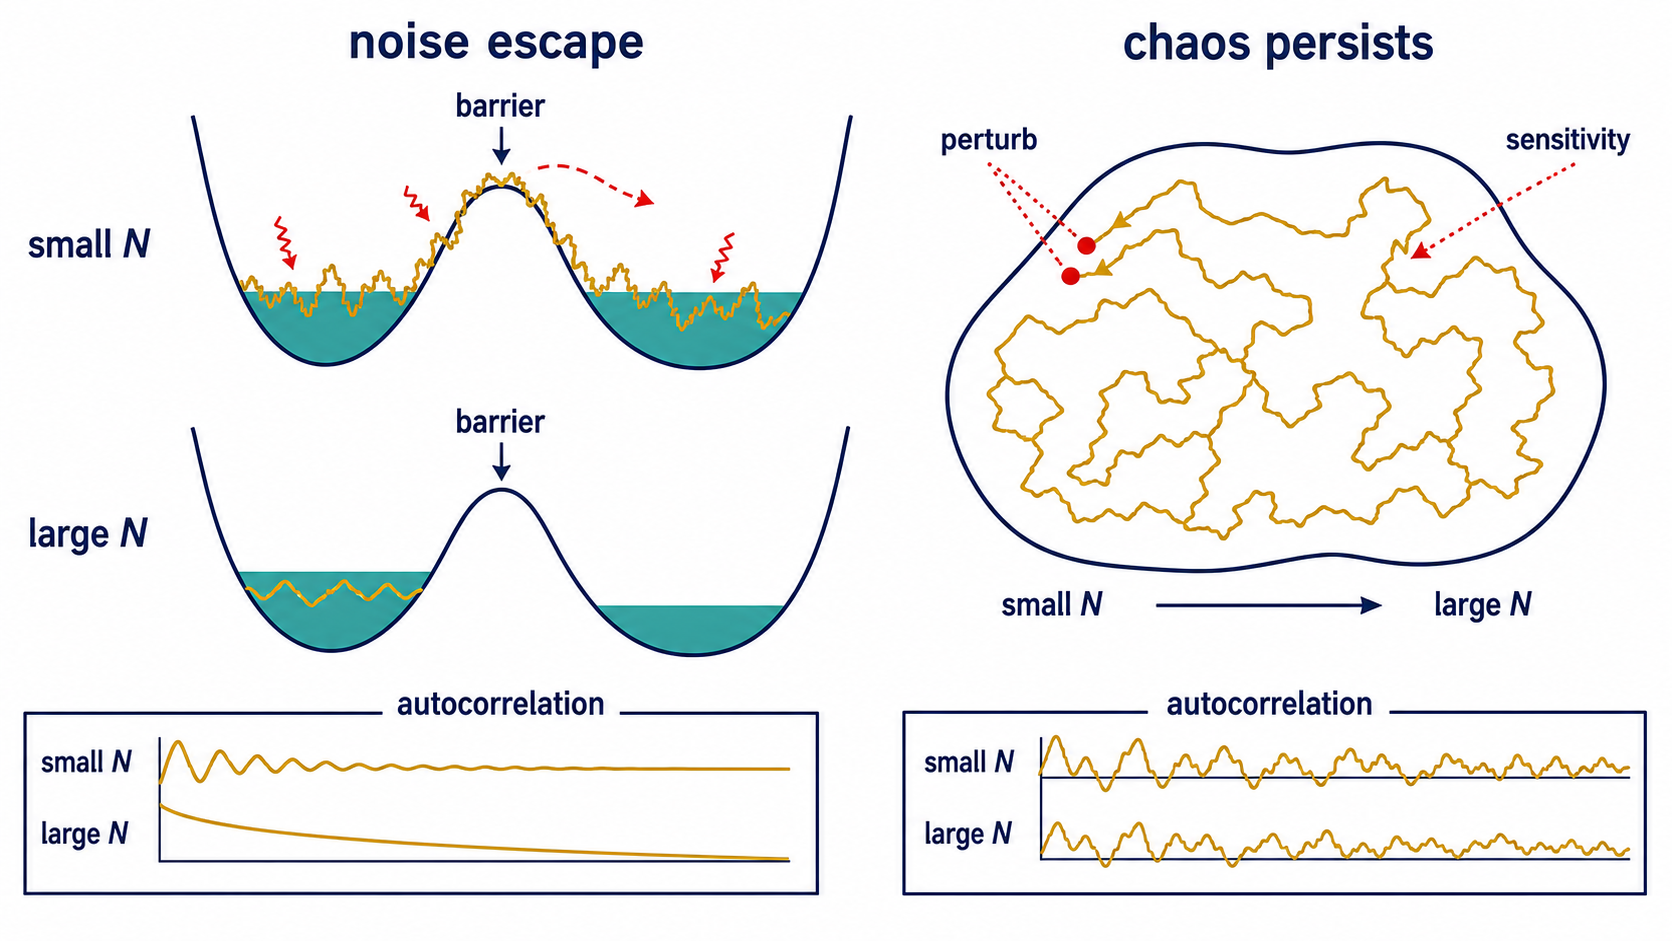
\includegraphics[width=0.95\textwidth]{figures/meso-noise-escape-vs-chaos.png}
\caption{Noise-driven metastability and mesoscopic chaos make different finite-size predictions. If switching is escape over a barrier, increasing population size suppresses the fluctuations that drive transitions. If the mesoscopic equations are chaotic, irregular wandering and perturbation sensitivity can remain in the large-population limit.}
\label{fig:noise-escape-vs-chaos}
\end{figure}

% ============================================================
\section{How to distinguish finite-size switching from deterministic or chaotic switching}
\label{sec:distinguish-finite-size-chaotic-switching}
% ============================================================

The core theory question is whether slow cluster switching is best understood as stable attractors plus finite-size noise, or as deterministic irregular dynamics at the mesoscopic level. These mechanisms can look similar in a raster plot. They make different scaling and perturbation predictions.

\subsection{Network-size scaling}

If switching is driven by intrinsic finite-size noise, increasing cluster size while holding the deterministic mean-field parameters fixed should reduce switching. A schematic prediction is
%
\begin{equation}
  \log T_{\mathrm{dwell}}(N)
  \approx
  aN+b
  \label{eq:dwell-log-linear-size}
\end{equation}
%
for a rare-event regime with a fixed barrier. The constants $a$ and $b$ depend on the barrier and noise covariance. The exact form may deviate from this simple line, but dwell times should grow strongly with $N$.

If switching is deterministic chaos in a mesoscopic system, increasing microscopic neuron number should reduce sampling noise but should not remove the deterministic irregular switching. Dwell statistics should approach a nontrivial large-$N$ limit.

\subsection{Lyapunov exponents}

Deterministic chaos requires sensitive dependence on initial conditions. In a deterministic mesoscopic model
%
\begin{equation}
  \dot{\vec R}=\vec f(\vec R),
  \label{eq:ch09-deterministic-mesoscopic-system}
\end{equation}
%
the maximal Lyapunov exponent is
%
\begin{equation}
  \lambda_{\max}
  =
  \lim_{t\to\infty}
  \frac{1}{t}
  \log
  \frac{\|\delta \vec R(t)\|}{\|\delta \vec R(0)\|}.
  \label{eq:max-lyapunov}
\end{equation}
%
If $\lambda_{\max}>0$ in the large-population deterministic limit, nearby trajectories separate exponentially and chaos is plausible. If all Lyapunov exponents are negative around attractors and switching disappears as $N$ grows, a finite-size escape picture is more plausible.

\subsection{Clone and common-noise tests}

Run two simulations from nearly identical mesoscopic states. If deterministic chaos dominates, tiny perturbations should grow even without changing the random seed. If finite-size noise dominates, two simulations with the same stochastic increments should remain close longer than two simulations with independent stochastic increments.

A useful protocol is:
%
\begin{enumerate}[leftmargin=*]
  \item initialize two copies at the same cluster state;
  \item run them with identical quenched connectivity;
  \item compare independent dynamic noise, shared dynamic noise, and no dynamic noise;
  \item measure divergence time and transition times.
\end{enumerate}
%
This separates sensitivity to deterministic initial conditions from sensitivity to stochastic spike-count fluctuations.

\subsection{Autocorrelation and dwell-time signatures}

Noise-driven switching among stable states often produces approximately exponential dwell-time distributions when escape is memoryless within a basin:
%
\begin{equation}
  \Pr(T_{\mathrm{dwell}}>t)
  \approx
  \exp(-t/\tau_{\mathrm{escape}}).
  \label{eq:ch09-exponential-dwell-survival}
\end{equation}
%
The autocorrelation of a two-state observable then has a slow component set by transition rates.

Deterministic chaotic switching may produce broader or more structured dwell-time distributions, especially if trajectories follow preferred channels or visit unstable remnants of attractors. This is not a definitive test by itself, but it is useful when combined with size scaling and perturbation response.

\subsection{Perturbation-response tests}

For noise-driven attractor switching, a small pulse near a basin boundary can strongly change transition probability, while the same pulse deep inside a basin may decay. The response depends on where the state lies relative to the separatrix.

For deterministic chaotic switching, perturbations may change phase along an irregular trajectory rather than simply pushing the system over a barrier. Repeated pulse experiments should therefore be aligned to state-space position, not only clock time.

The practical diagnostic is to reconstruct a low-dimensional mesoscopic state, estimate where transitions occur, and test whether transitions concentrate near basin boundaries predicted by a deterministic drift. If they do, finite-size escape is plausible. If the deterministic drift itself contains an irregular attractor with positive Lyapunov exponent, mesoscopic chaos becomes plausible.

\begin{chaptersummary}

\begin{center}
\renewcommand{\arraystretch}{1.55}
\begin{tabularx}{\textwidth}{@{}l X X@{}}
  \toprule
  \textbf{Concept} & \textbf{Equation} & \textbf{Key prediction} \\
  \midrule
  Mesoscopic Langevin equation &
  $\dd\vec R=\vec f(\vec R)\dd t+N^{-1/2}\mat G(\vec R)\dd\vec W_t$ &
  Drift plus finite-size fluctuations \\
  Intrinsic count noise &
  $\Var[\widehat A_\alpha]=r_\alpha/(N_\alpha\Delta t)$ &
  Activity noise shrinks as $N_\alpha^{-1/2}$ \\
  Multiplicative noise &
  $\E[\dd R_\alpha\dd R_\beta]\propto [\mat G\mat G^\top]_{\alpha\beta}\dd t/N$ &
  Noise amplitude and direction depend on state \\
  Quenched disorder &
  $W^{(m)}=\bar W+\Delta W^{(m)}$ &
  Fixed network realization changes drift and basin depths \\
  Coherent mode &
  $R_{\mathrm{com}}=C^{-1}\sum_\alpha R_\alpha$ &
  Shared fluctuations move many clusters together \\
  Escape scaling &
  $T\approx C\exp(N\Delta U/D)$ &
  Finite-size switching becomes rare as $N$ grows \\
  Chaos test &
  $\lambda_{\max}>0$ &
  Deterministic irregularity persists without finite-size noise \\
  \bottomrule
\end{tabularx}
\end{center}

\end{chaptersummary}

\begin{conceptquestions}
  \item In the Langevin equation, which term determines fixed points and which term determines finite-size wandering around them?
  \item Why is spiking population noise usually multiplicative rather than additive?
  \item Give one experimental or simulation statistic that separates quenched disorder from dynamic noise.
  \item What is the difference between a coherent fluctuation and an incoherent cluster-contrast fluctuation?
  \item Why does Kramers-like escape predict a strong dependence of dwell time on population size?
  \item What would you expect to happen to switching if cluster size is doubled under a finite-size escape hypothesis?
  \item Why is a positive maximal Lyapunov exponent evidence for deterministic chaos rather than ordinary noise-driven switching?
  \item Design a clone simulation that uses common noise to distinguish deterministic sensitivity from stochastic sensitivity.
  \item Why are dwell-time distributions useful but not sufficient for deciding between finite-size switching and mesoscopic chaos?
\end{conceptquestions}
